\section{Java EE und Microservices}
Aus rein technologischer Sicht bietet Java EE alles, was für eine Microservice-basierte Architektur erforderlich ist. Das wird bereits klar, wenn die verfügbaren APIs betrachtet werden \cite{jaxcenter.2016}. Microservices ergeben sich unter Berücksichtigung folgenden Eigenschaften, welche zudem Indikatoren für die Größe darstellen [5].
\begin{itemize}
	\item Teamgröße
	\item Modularisierung
	\item Ersetzbarkeit
	\item Transaktionen und Konsistenz
	\item Infrastruktur
	\item Verteilte Kommunikation	
\end{itemize}
Soll nun ein Microservice mit Java EE implementiert werden, lassen sich diese Indikatoren ebenfalls heranziehen. Die Anzahl der Teammitglieder beschränkt die Größe der Komponente. Sie beinhaltet dabei so viel Logik, dass sie von einem Team entwickelt und betrieben werden kann. Microservices sollen eine geschlossene Fachlichkeit abbilden (Bounded Context), um sich eindeutig von anderen Services abzugrenzen. Durch diesen fachlich orientierten Aufbau, lässt sich der Dienst unabhängig von anderen Teams implementieren, testen und in Produktion bringen. Auch die Komplexität ist handhabbar, wenn der Service als Modul entwickelt wird und lässt sich somit auch ersetzen, sollte dies von Nöten sein. Die Transaktion, welche die ACID-Eigenschaften verfolgt, kann ebenfalls entsprechend implementiert werden. Die Kommunikation über leichtgewichtige Mechanismen ergibt sich durch diesen Ansatz [5]. Da sie Teil eines verteilten Systems sind, bedienen sich über die verteilte Kommunikation einer anderen Fachlichkeit oder stellen anderen Services die eigene zur Verfügung.  \\ 
Diesen Anforderungen genügt Java EE bereits. Microservices lassen sich mit den vorhandenen APIs problemlos erstellen. Über JAX-RS (Java API for RESTful Web Services) lässt sich die Kommunikation der Dienste realisieren. Über Bean Validation (Java EE-Standard für eine schichtenübergreifende Validierung) können Requests auf ihre Korrektheit überprüft werden. Die Nutzlast kann beispielsweise über JSON-P entsprechend umgewandelt werden, um die Übermittlung zu ermöglichen. Die fachliche Logik innerhalb des Dienstes sowie die Datenhaltung lässt sich über CDI (Context and Dependency Injection) sowie JPA (Java Persistence API) realisieren [x]. Selbst NoSQL-Datenbanken können über entsprechende Bibliotheken an das System angebunden werden. Auch eine eigene Benutzeroberfläche lassen sich in solche Anwendungen integrieren, wie es bei Microservices priorisiert wird. Es ist also nicht der Fall, dass ein Service, welcher über das Java EE Framework entwickelt wurde, automatisch eine aufgeblähte Mehrschichtenarchitektur mit sich bringt, welche entsprechende Methodenaufrufe nur über Dependency Injection Schicht für Schicht weiter delegiert. Durch verwenden entsprechender Features lassen sich sehr effiziente und schlanke Architekturen realisieren \cite{jaxcenter.2016}.\\
Microservice-basierte Anwendungen sind Applikationen, die sich aus einer Reihe von kleinen Komponenten zusammensetzen. Diese durchlaufen dabei alle ihre eigenen Prozesse. Somit ist ein weiterer, zu berücksichtigender Punkt, die Infrastruktur. Jede Einheit muss unabhängig deployt werden können. Hierfür gibt es die Continuous-Delivery-Pipelne, die durch eine weitgehende Automatisierung dafür sorgt, dass Software bereitgestellt werden kann. Jeder Dienst benötigt somit eine eigene Infrastruktur, um ihn auszuführen. Diese kann auch Datenbanken oder Application Server beinhalten [5]. Hier ergibt sich allerdings ein Problem mit Enterprise Java.

\section{Das Problem mit Java EE}
Die oben aufgeführten Punkte sind Ansätze für Continuous Delivery. Diese Disziplin erfolgt durch eine weitgehende Automatisierung entsprechender Prozesse. Das eigentliche Problem liegt nicht in der zu verwendenden Technologie bzw. dem reinen Entwickeln, es geht um die potenzielle Automatisierung dieser Entwicklung. Auch zur Laufzeit zeigen sich Probleme. Das Vorgehen für Build und Deployment, welches in Java EE-Anwendungen vorgesehen ist, geht über das Zusammenpacken der Komponenten, die dann in einem Application Server deployt werden (siehe Abbildung ...). Die notwendige Infrastruktur wird von diesem Server bereitgestellt [x]. Eine Skalierung, die eine anfallende Last pro Fachlichkeit ausgleicht, kann somit nur sehr umständlich erreicht werden. Bei Anwendungen, die auf Microservices basieren, geht es teilweise um tausende Serverinstanzen mit zigtausend Deployments pro Jahr (laut Amazon sogar etliche Millionen). Dies mit Java EE zu bewerkstelligen stellt sich dabei als sehr schwer heraus. Dafür sind entsprechende Server nicht schnell genug, denn der durch Java-EE anfallende Overhead an zu unterstützenden APIs und Features ist zu groß bzw. die Anwendungsserver einfach zu schwerfällig  \cite{jaxcenter.2016}. \\ 
Leichtgewichtige Server, die nur Bestandteile mit sich bringen, welche für den Service benötigt werden, würden Abhilfe schaffen \cite{jaxcenter.2016}. Denkbar wäre hier als erster Ansatz das separate Packen der Anwendungen, welche anschließend auf dem Server deployt werden. Die durch den Server können sich die Dienste die zur Verfügung gestellte Infrastruktur teilen. Microservices sollen allerdings alle in einem eigenen Prozess unabhängig voneinander laufen. Diese Unabhängigkeit kann durch den eben genannten Ansatz nicht realisiert werden. Das Deployment eines Service würde das Laufzeitverhalten der anderen Dienste beeinflussen. Fällt der Server aus oder weist ein Fehlverhalten durch einen defekten Service auf, können die anderen Dienste ebenfalls nicht mehr erreicht werden [x].\\
\begin{figure}[h!]
	\centering
	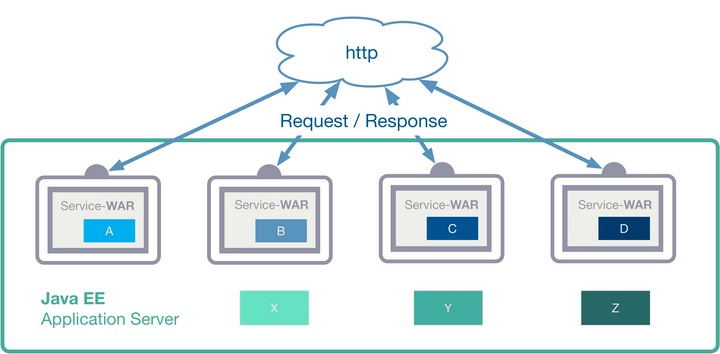
\includegraphics[width=1.0\linewidth]{images/mp1}
	\caption{Deployment in Application Server [x]}
	\label{fig:mp1}
\end{figure}

\section{Die Optimierung von Java EE}
Um Dienste auf Basis von Java EE bezüglich der Unabhängigkeit zu optimieren, wäre es denkbar jede Komponente in einen eigenen Server zu deployen. Jeder Dienst hat somit seine eigene Infrastruktur. Dies wird in Abbildung (...) illustriert. Wie bereits erwähnt handelt es sich bei Microservice-basierten Systemen oft um etliche Service-Instanzen und deployments. Durch die angestrebte Automatisierung über die Delivery-Pipeline wären operative Aufwände wie Deployment, Konfiguration etc. zu stemmen. Automatisierung kann beispielsweise durch das Einbetten in Docker-Images erreicht werden. Allerdings ergeben sich auch hier Probleme zur Laufzeit. Der Ressourcenverbrauch der Dienste treibt die Last auf den Servern entsprechend in die Höhe.
  

%Die Arbeit lehnt sich dabei an die von Lars Röwekamp verfassten Artikel auf diversen Plattformen an. Durch seine Beiträge manifestierte er seine grenzenlose Inkompetenz. Scheiß auf dich und dein Copyright.
\begin{figure}[h!]
	\centering
	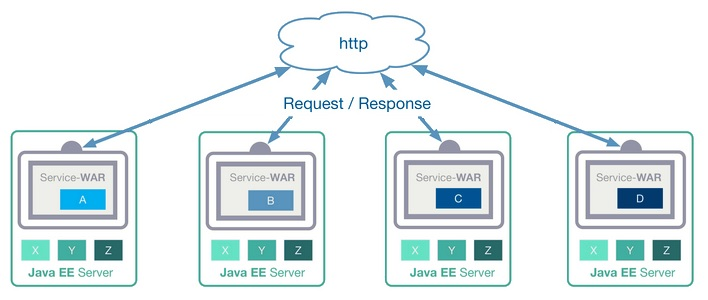
\includegraphics[width=1.0\linewidth]{images/mp2}
	\caption{Dienste mit eigener Infrastruktur [x]}
	\label{fig:mp2}
\end{figure}


Führende Application-Server-Hersteller (WildFly Swarm, TomEE etc.) sind bereits daran entsprechende Varianten zu entwickeln \cite{LarsRowekamp.2016}. Dabei sollen Bestandteile und Funktionalitäten des Servers in den Service eingebunden werden \cite{jaxcenter.2016}.


Somit erhält man einen fachlich abgekapselten Service, der zudem seine eigene Laufzeitumgebung mit sich bringt. Diese Umgebung kann dabei entsprechend auf den Service angepasst werden, wodurch der Overhead hier auch drastisch reduziert werden kann. Sobald dieser Service nun deployt wird, kann er gestartet und ausgeführt werden. Er ist autark und läuft als eigener Prozess. Allerdings ist dieser Ansatz noch etwas zu grobgranular. Von einem Self-contained System (SCS) ist hier somit eher die Sprache \cite{jaxcenter.2016}. Dieser Ansatz teilt sich zwar eine Vielzahl von Konzepten mit Microservices (Isolation, unabhängige Einheiten, fachliche Trennung, Technologiefreiheit, keine zentrale Infrastruktur), besitzt jedoch noch einige Unterschiede zum feingranularen Ansatz der Microservices. Wie eben bereits hervorgegangen ist, weist bereits die Größe ein Unterschied auf. Ein System besitzt normalerweise weniger SCS als Microservices. Ein wichtiger Aspekt ist die Kommunikation zwischen den Komponenten. Microservices können untereinander kommunizieren. SCSs sollten dies idealerweise nicht. Auch bringen Microservices oft ihre eigene Benutzeroberfläche mit sich, während sich SCSs eine gemeinsame teilen. Es wird an dieser Stelle also nicht das gewünschte Problem gelöst. SCSs sind eher für Architekturen größerer Projekte gedacht \cite{selfcontainedservices.2017}. Sollen noch unabhängigere, kleinere Komponenten entwickelt werden, die auch mit Continuous Delivery arbeiten, muss noch ein Schritt weitergegangen werden. 